\documentclass[11pt]{article}
\usepackage[margin=1in]{geometry}
\usepackage{graphicx}
\usepackage{enumitem}
\usepackage{parskip}

\title{TA Onboarding}
\author{}
\date{}

\begin{document}

\maketitle

\section*{Current Status}
Verified on March 16, 2026 against the live Supabase-backed portal.

Smoke-tested TA workflows:
\begin{itemize}
  \item login and assigned-cohort dashboard load
  \item session checklist update
  \item handoff note creation
  \item messaging access
  \item direct access to \texttt{/billing} correctly redirected back to \texttt{/dashboard}
\end{itemize}

\section*{What TA Is For}
TA is the assigned-cohort support role.

TA owns:
\begin{itemize}
  \item classroom support for assigned cohorts
  \item attendance support context
  \item session checklist updates
  \item handoff notes for instructors
  \item limited family messaging inside assigned cohorts
\end{itemize}

TA does not own:
\begin{itemize}
  \item billing
  \item settings
  \item integrations
  \item global cohort management
  \item saved views or personal templates
\end{itemize}

\section*{Core Boundaries}
TA can:
\begin{itemize}
  \item access \texttt{dashboard}, \texttt{calendar}, \texttt{cohorts}, \texttt{attendance}, \texttt{students}, \texttt{families}, \texttt{academics}, and \texttt{messaging}
  \item work only inside assigned cohorts
  \item see contact basics for those families
  \item create classroom-support notes and flags
  \item update assigned tasks, academic notes, resources, and same-day score context inside assigned cohorts
  \item use category-guarded family threads for assigned cohorts
\end{itemize}

TA cannot:
\begin{itemize}
  \item open \texttt{billing}, \texttt{integrations}, \texttt{programs}, or \texttt{settings}
  \item perform bulk operations
  \item change staffing or cohort structure
  \item export data
  \item use engineer or admin-only tooling
\end{itemize}

\section*{Screens}
\subsection*{TA Dashboard}
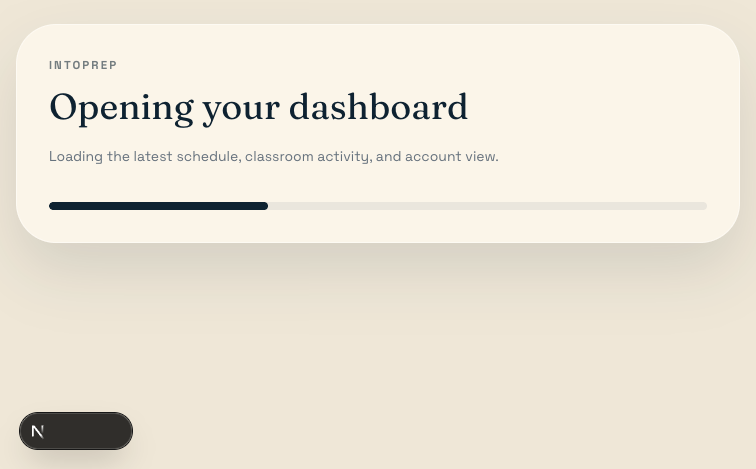
\includegraphics[width=\textwidth]{assets/ta-dashboard.png}

\subsection*{TA Attendance}
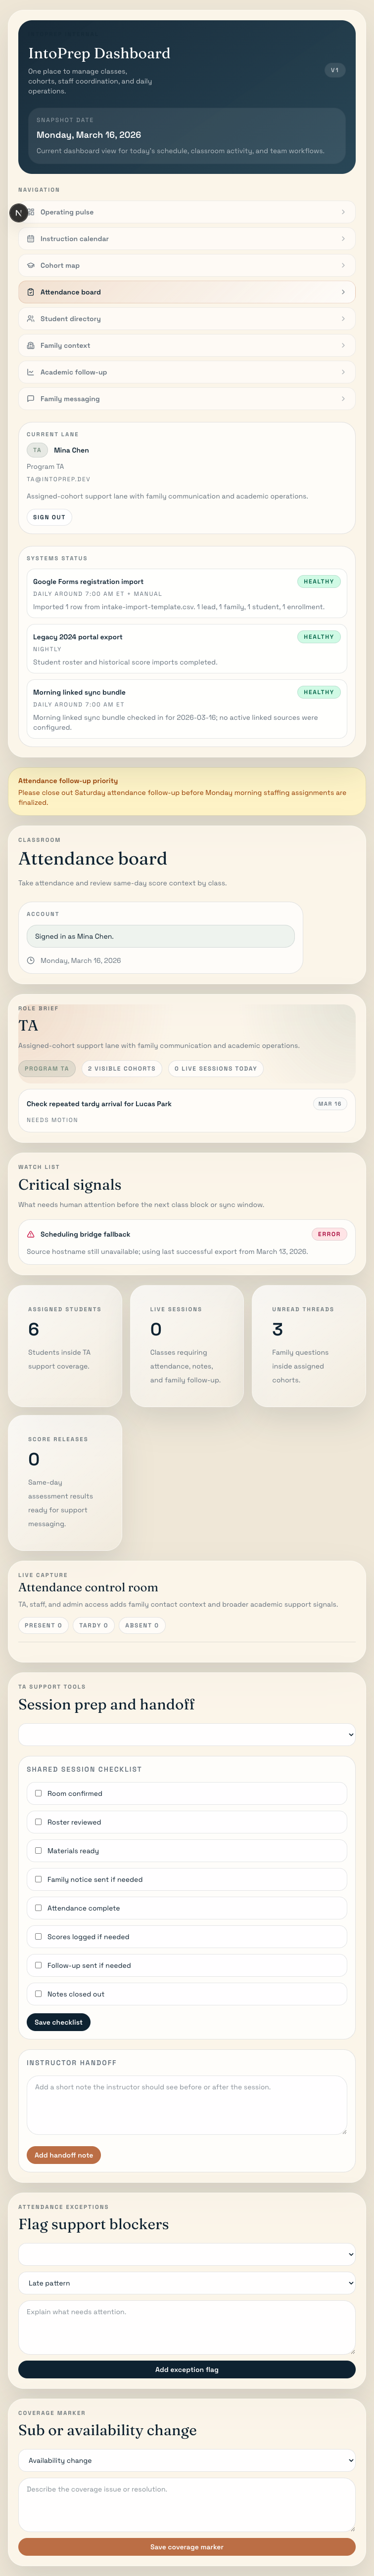
\includegraphics[width=\textwidth]{assets/ta-attendance.png}

\subsection*{TA Messaging}
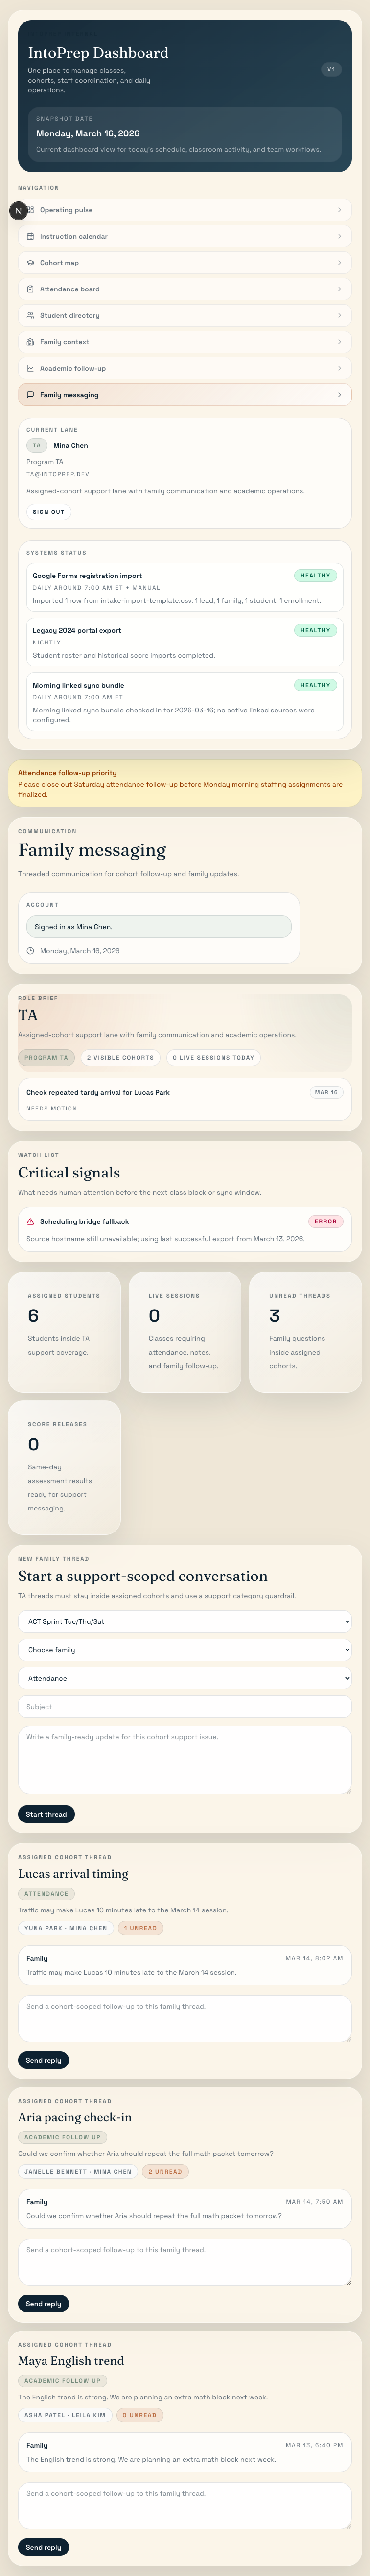
\includegraphics[width=\textwidth]{assets/ta-messaging.png}

\section*{First Login Walkthrough}
\begin{enumerate}
  \item Sign in at \texttt{/login}.
  \item Start on ``Operating pulse''.
  \item Review:
  \begin{itemize}
    \item assigned tasks
    \item today’s sessions
    \item unread family threads
    \item blocker or handoff items
  \end{itemize}
  \item Open ``Attendance board''.
  \item Open ``Family messaging'' only for assigned families and read the current thread context before sending anything.
\end{enumerate}

\section*{Daily Workflow}
\subsection*{1. Start With The Dashboard}
Use the dashboard to decide:
\begin{itemize}
  \item which session needs attention first
  \item which task is blocked
  \item which family thread needs an answer
\end{itemize}

\subsection*{2. Prepare And Close Out Sessions}
Open ``Attendance board'' for each assigned session.
\begin{itemize}
  \item check rosters
  \item update shared checklist items
  \item log handoff notes for the instructor
  \item keep attendance-related follow-up visible
\end{itemize}

Smoke test verification:
\begin{itemize}
  \item TA checklist update succeeded
  \item TA handoff note creation succeeded
\end{itemize}

\subsection*{3. Support Family Communication Carefully}
Open ``Family messaging'' to:
\begin{itemize}
  \item reply to existing cohort-scoped threads
  \item start a one-off thread only when it belongs to an allowed category such as attendance, scheduling, or academic follow-up
\end{itemize}

\subsection*{4. Stay Inside Your Cohorts}
You should only see the cohorts assigned to you. If a cohort or family is missing, it is usually an assignment problem, not a page bug.

\section*{Complete Capability Map}
TA is the classroom-support role for assigned cohorts only.

Use TA for:
\begin{itemize}
  \item assigned tasks
  \item attendance support
  \item shared session checklists
  \item instructor handoff notes
  \item attendance exception flags
  \item coverage and availability markers
  \item academic notes, resources, and same-day score support in assigned cohorts
  \item read-only student trend review
  \item family threads for allowed support categories
\end{itemize}

Do not use TA for:
\begin{itemize}
  \item billing
  \item global operations
  \item staffing or capacity changes
  \item settings or integrations
  \item bulk messaging
  \item family contact-history logging outside the thread workflow
\end{itemize}

\section*{How To Update A Session Checklist}
\begin{enumerate}
  \item Open the session from ``Attendance board''.
  \item Review the prep and closeout items.
  \item Update the checklist state for items that are complete.
  \item Save the checklist so staff and admin see the updated classroom state.
\end{enumerate}

Typical checklist items include:
\begin{itemize}
  \item room confirmed
  \item roster reviewed
  \item materials ready
  \item attendance complete
  \item follow-up sent if needed
\end{itemize}

\section*{How To Leave A Handoff Note}
\begin{enumerate}
  \item Open the assigned session.
  \item Add the handoff note after class or when context changes.
  \item Keep it short and operational.
  \item Focus on what the instructor needs next, not general narrative.
\end{enumerate}

Good handoff notes mention:
\begin{itemize}
  \item pacing issues
  \item attendance oddities
  \item student support needs
  \item what was already handled
\end{itemize}

\section*{How To Use Attendance Exception Flags}
\begin{enumerate}
  \item Open the assigned session in ``Attendance board''.
  \item Choose the student row that needs attention.
  \item Add the right flag type, such as repeated lateness or missing guardian reply.
  \item Add a short operational note that helps staff or admin continue the follow-up.
\end{enumerate}

\section*{How To Use Coverage Markers}
\begin{enumerate}
  \item Open the assigned session.
  \item Add a coverage or availability marker only when the class team needs to know about a support-gap risk.
  \item Keep the note brief and operational.
  \item Do not treat this as a staffing-change tool. It is a visibility tool.
\end{enumerate}

\section*{How To Work Academics As A TA}
\begin{enumerate}
  \item Open ``Academic follow-up'' for your assigned cohort.
  \item Add or update same-day academic notes as needed.
  \item Publish resources only within your assigned cohort workflows.
  \item Review trends read-only to understand where students may need support.
\end{enumerate}

\section*{How To Start A TA Family Thread}
\begin{enumerate}
  \item Open ``Family messaging''.
  \item Confirm the family is inside one of your assigned cohorts.
  \item Choose the allowed thread category:
  \begin{itemize}
    \item attendance
    \item scheduling
    \item academic follow-up
  \end{itemize}
  \item Write the message clearly and keep it inside the classroom-support lane.
\end{enumerate}

\section*{How To Work TA Tasks}
\begin{enumerate}
  \item Start from the dashboard task queue.
  \item Update only tasks assigned to you.
  \item Use progress, handoff, or blocker notes to keep staff and admin informed.
  \item If the work needs authority beyond TA scope, stop and hand it off rather than improvising outside role boundaries.
\end{enumerate}

\section*{Messaging Rules}
\begin{itemize}
  \item stay within assigned cohorts
  \item use only allowed support categories
  \item do not discuss billing
  \item do not use TA role for broad operational messaging
\end{itemize}

\section*{Guardrails}
\begin{itemize}
  \item no direct billing access
  \item no settings access
  \item no integrations access
  \item no saved views or personal templates
  \item no staffing or cohort structure changes
\end{itemize}

\section*{Verified Behavior}
Verified in the live browser pass:
\begin{itemize}
  \item TA login succeeded
  \item dashboard, attendance, and messaging loaded
  \item checklist update succeeded through the live API
  \item handoff note creation succeeded through the live API
  \item direct access to \texttt{/billing} redirected back to \texttt{/dashboard}
\end{itemize}

\section*{Recommended First-Day Checklist}
\begin{itemize}
  \item review your dashboard
  \item open one assigned session in attendance
  \item update a checklist item in demo data
  \item leave a sample handoff note
  \item read existing family threads before sending anything new
\end{itemize}

\end{document}
\ No newline at end of file
